\section{考生开展本课题研究的主要思路、基本内容和重要观点}\label{sec:2.4}
在大数据的背景下, 面对非平稳状态下动态机制不确定和高复杂度的大规模时间序列数据,
本课题认为建立一种具有普适逼近能力的、基于随机分布统计视角的和可解释可自适应调整的神经网络学习模型
能够有效地学习时间序列数据的状态与规律。基于此,本课题具有重要的理论与实际意义。
\begin{figure*}[ht]
    \centering
    \begin{minipage}{0.5\textwidth}
        \centering
        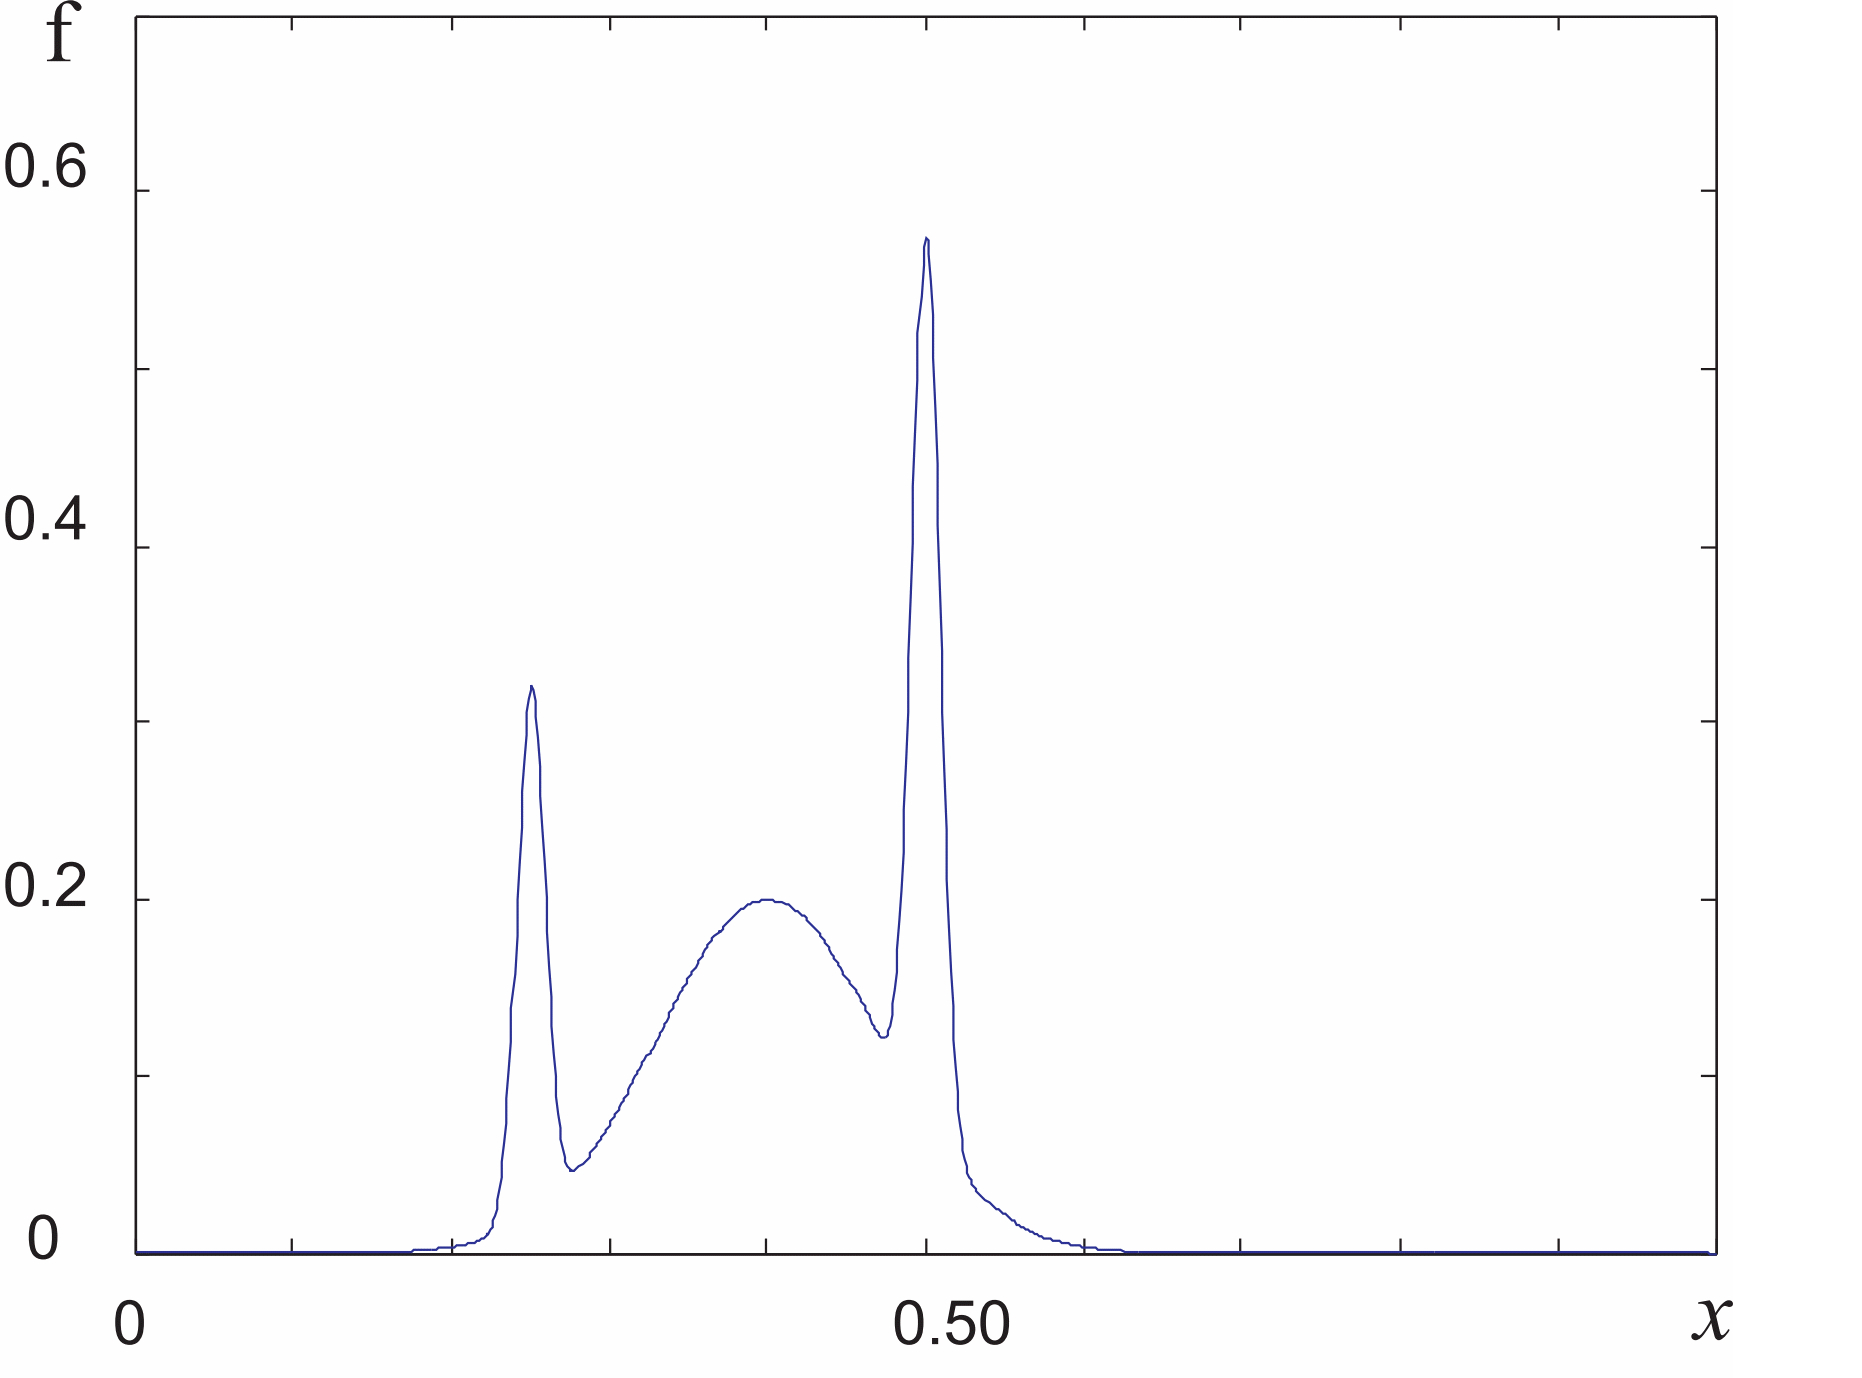
\includegraphics[width=0.6\textwidth]{data.png}
        \caption{\label{fig:data} 时间数据数据示例}
    \end{minipage}%
    \begin{minipage}{0.5\textwidth}
        \centering
        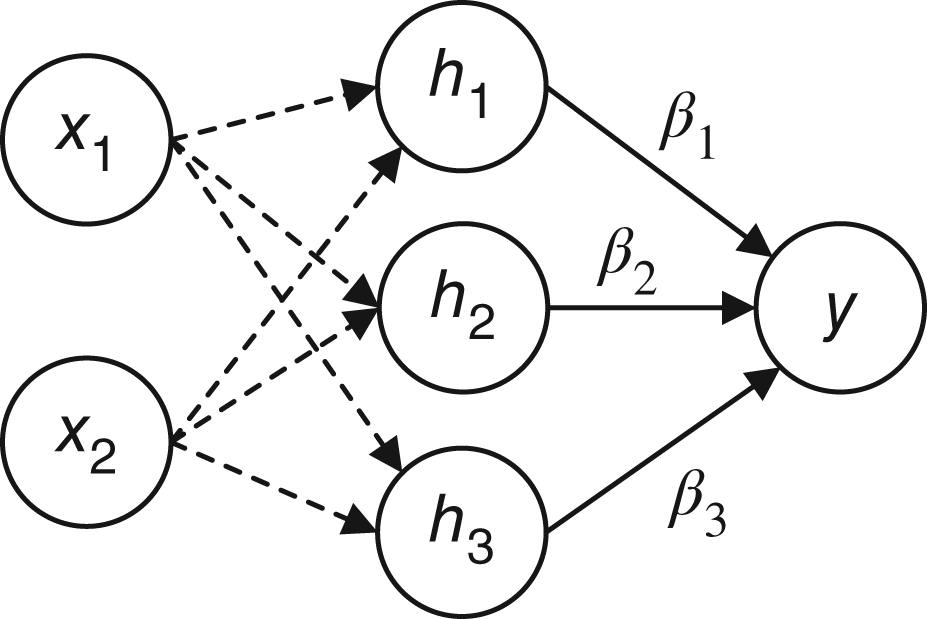
\includegraphics[width=0.6\textwidth]{network.png}
        \caption{\label{fig:network} 神经网络示例}
    \end{minipage}%
\end{figure*}

对于如\autoref{fig:data}所示的时间序列数据示例,其公式为$f(x)=0.2e^{-(10x-4)^{2}}+0.5e^{-(80x-40)^{2}}+0.3e^{-(80x-20)^{2}}$
。这类时间序列数据在金融市场和故障监测等实际情景中极为常见,
其在某一区域内剧烈波动的状态难以被传统的非线性回归方法逼近。
神经网络作为多重感知机,可以凭借其不同的基函数与非线性激活函数的组合了理论上拟合出这类不平稳且局部高复杂度的函数。
但在实际应用确定神经网络模型去逼近此类函数时,亦有明显的缺陷和问题。
首先确定神经网络模型需要经过多次的实验比较来调整神经网络的层数、各层隐藏层神经元数量和激活函数类型等参数,
这一过程非常耗费研究人员或工作人员的精力同时对于不同的时间序列数据需要重复调参来优化神经网络的逼近效果;
另一方面,在采用梯度下降算法进行逼近收敛时,无法保证收敛速度;
且在此过程中,无法解释神经网络中神经单元作用,即无法得知在网络优化中各层各神经单元对整体网络优化的影响。
这些缺陷和问题制约了时间序列数据的逼近研究,基于此,本课题研究一个具有普适能力,神经网络权重分布可知和
可根据不同时间序列数据自适应调整网络结构的神经网络学习模型,并给出了理论证明。

对于如\autoref{fig:network}所示的神经网络示例,$X_i$表示输入层的时间序列数据,该数据具有$d$维特征;
$h_q$表示隐藏层单元,该隐藏层神经元有$m$个,每个神经元可表示为$g(w^\mathrm{T}x+b)$;
$\beta$表示隐藏层单元的输出矩阵;
$Y$表示输出层的时间序列数据。

在进行时间序列数据驱动下的可解释学习模型证明前,首先对模型中的函数条件、范式和内积进行约束和定义。
在时间序列数据的范畴下,模型中的函数均为勒贝格测度函数(Lebesgue measurable functions)且均为实值函数。
在此,以$\Gamma:=\{g_1, g_2, g_3...\}$表示一组实值函数,span$(\Gamma)$表示由$\Gamma$张成的函数空间;
$L_{2}(D)$ 表示包含所有勒贝格测度函数$f=[f_1,f_2,\ldots,f_m]:\mathbb{R}^{d}\rightarrow \mathbb{R}^{m}$, $D\subset \mathbb{R}^{d}$的函数空间;
$L_2$范式被定义为:
\begin{equation}\label{multiple_lp}
    \|f\|:=\left(\sum_{q=1}^{m}\int_{D}|f_q(x)|^2dx\right)^{1/2}<\infty
  \end{equation}

勒贝格测度函数的内积被定义为:
\begin{equation}\label{multiple_inner}
    \langle f,\theta\rangle:=\sum_{q=1}^{m}\langle f_q,\theta_q\rangle=\sum_{q=1}^{m}\int_{D}f_q(x)\theta_q(x)dx
  \end{equation}

在$m=1$的特殊情况下,
对于一个实值函数 $\psi:\mathbb{R}^{d}\rightarrow \mathbb{R}$, $D\subset \mathbb{R}^{d}$,
其$L_2$范式为$ \|\psi\|:=(\int_{D}|\psi(x)|^2dx)^{1/2}$,
其内积为$\langle \psi_1,\psi_2\rangle=\int_{D}\psi_1(x)\psi_2(x)dx$。

在时间序列数据驱动下的可解释学习模型中,对于一个目标函数$f:\mathbb{R}^{d}\rightarrow \mathbb{R}^{m}$,
假设已经产生了$L-1$层隐藏层单元,即$f_{L-1}(x)=\sum_{j=1}^{L-1}\beta_jg_j(w_j^\mathrm{T}x+b_j)$ ($L=1,2,\ldots$, $f_0=0$),
其中$\beta_j=[\beta_{j,1},\ldots,\beta_{j,m}]^\mathrm{T}$。
学习模型的残差可表示为$e_{L-1}=f-f_{L-1}=[e_{L-1,1},\ldots,e_{L-1,m}]$。
若$\|e_{L-1}\|$未达到预定的误差范围, 此时该学习模型的学习能力不够,
需要继续生成一个隐藏层单元即随机基函数$g_L$ ($w_L$ and $b_L$)并计算或优化其输出权重$\beta_L$,
通过这种方式学习模型的残差$f_{L}=f_{L-1}+\beta_Lg_L$将进一步缩小。
在本课题研究中,学习模型的随机权重将受到约束并保证普适逼近能力。

对此,有基准的学习模型I。假设span($\Gamma$)在$L_2$空间中是密集的,且$\forall g\in \Gamma$, $0<\|g\|<b_g$, $b_g\in \mathbb{R}^{+}$。
有[0-1]区间的学习速率$r, 0<r<1$和非负实数序列$\{\mu_L\}$且$\lim_{L\rightarrow+\infty}\mu_L=0$, 
$\mu_L\leq (1-r)$。
对于隐藏层神经元$L=1,2,\ldots$, 有:
\begin{equation}\label{delta1}
    \delta_{L}=\sum_{q=1}^{m}\delta_{L,q}, \delta_{L,q}=(1-r-\mu_L)\|e_{L-1,q}\|^2, q=1,2,...,m
    \end{equation}

若随机基函数$g_L$在满足以下不等式约束的前提下生成:
\begin{equation}\label{step1}
    %\sum_{q=1}^m\langle e_{L-1,q},g_L\rangle^2\geq b_g^2\delta_L,
    \langle e_{L-1,q},g_L\rangle^2\geq b_g^2\delta_{L,q}, q=1,2,...,m
    \end{equation}

且输出权重由以下公式计算得出:
\begin{equation}\label{step2}
    \beta_{L,q}=\frac{\langle e_{L-1,q},g_L\rangle}{\|g_L\|^2}, q=1,2,\ldots,m
    \end{equation}

则可得出此学习模型具有普适逼近能力,即$\lim_{L\rightarrow +\infty}\|f-f_L\|=0,$
其中$f_L=\sum_{j=1}^{L}\beta_{j}g_j$, $\beta_j=[\beta_{j,1},\ldots,\beta_{j,m}]^{\mathrm{T}}$。

该普适逼近能力可被证明为:根据\autoref{step2},可以验证其残差$\{\|e_{L}^2\|\}$是单调递减的。
因此,$\{\|e_L\|\}$在$L\rightarrow +\infty$时收敛。根据\autoref{delta1}、\autoref{step1}和\autoref{step2}
,有:
\begin{eqnarray}
    &&\|e_L\|^2-(r+\mu_L)\|e_{L-1}\|^2\nonumber\\&=& \sum_{q=1}^m\left(\langle e_{L-1,q}-\beta_{L,q}g_L,e_{L-1,q}-\beta_{L,q}g_L\rangle-(r+\mu_L)\langle e_{L-1,q},e_{L-1,q}\rangle\right)\nonumber\\
    &=&\sum_{q=1}^m\left((1-r-\mu_L)\langle e_{L-1,q},e_{L-1,q}\rangle-2\langle e_{L-1,q},\beta_{L,q}g_L\rangle+\langle\beta_{L,q}g_L,\beta_{L,q}g_L\rangle\right)\nonumber\\
    &=&(1-r-\mu_L)\|e_{L-1}\|^2-\frac{\sum_{q=1}^m\langle e_{L-1,q},g_L\rangle^2}{\|g_L\|^2}\nonumber\\
    &=&\delta_L-\frac{\sum_{q=1}^m\langle e_{L-1,q},g_L\rangle^2}{\|g_L\|^2}\nonumber\\
    &\leq& \delta_L-\frac{\sum_{q=1}^m\langle e_{L-1,q},g_L\rangle^2}{b_g^2}\leq0
    \end{eqnarray}

学习模型I提供了一个基于随机分布的可解释和可自适应调整网络结构的神经网络学习模型。
不同于梯度下降算法优化整个神经网络的权重,学习模型I通过\autoref{step1}的不等式约束为新增的隐藏层神经元搜索合适的随机权重$w_L$与偏置$b_L$。这类时间序列数据在金融市场和故障监测等实际情景中极为常见,
同时由于 $\Psi(w,b)=\sum_{q=1}^m\langle e_{L-1,q},g_L\rangle^2/\|g_{L}\|^2$在参数空间中为连续函数,满足\autoref{step1}约束的随机权重$w_L$与偏置$b_L$能够很快的被搜索出来。
在\autoref{step1}的约束下,学习模型I不能能够随机的产生隐藏层权重,并且能够在根据时间序列数据自适应调整网络结构的同时满足模型对时间序列数据的普适逼近能力。

在学习模型I中,隐藏层单元的输出权重$\beta_L=[\beta_{L,1},\ldots,\beta_{L,m}]^{\mathrm{T}}$由$\beta_{L,q}=\langle e_{L-1,q},g_L\rangle/\|g_L\|^2$由计算得出,并在之后的神经网络调整中保持不变。
考虑到这种确定方法可能会导致整个学习模型的收敛速度较慢,因此在学习模型I的基础上加以对输出权重计算方法可加以改进。
具体为,在每次生成新的隐藏层单元即随机基函数$g_j (j=1,2,\ldots,L)$后,对整个学习模型中隐藏层单元输出权重$\beta_1,\beta_2,\ldots,\beta_{L}$采用最小二乘法进行优化,以此加快学习模型的逼近收敛速度。
这种方法同样可以保证学习模型对时间序列数据的普适逼近能力。

对此,有改进的学习模型II。已优化后的输出权重可表示为
$[\beta_1^{*}, \beta_2^{*},\ldots,\beta_{L}^{*}]=\arg \min_{\beta}\|f-\sum_{j=1}^{L}\beta_jg_j\|$, $e_{L}^{*}=f-\sum_{j=1}^{L}\beta_j^{*}g_j=[e_{L,1}^{*},\ldots,e_{L,m}^{*}]$,
定义未优化输出权重为$\tilde{\beta}_{L,q}=\langle e_{L-1,q}^{*},g_L\rangle/\|g_L\|^2$, $q=1,\ldots,m$, $\tilde{e}_{L}=e_{L-1}^{*}-\tilde{\beta}_{L}g_L$,
其中$\tilde{\beta}_{L}=[\tilde{\beta}_{L,1},\ldots,\tilde{\beta}_{L,m}]^{\mathrm{T}}$且$e_0^{*}=f$。

假设span($\Gamma$)在$L_2$空间中是密集的,且$\forall g\in \Gamma$, $0<\|g\|<b_g$, $b_g\in \mathbb{R}^{+}$。
有[0-1]区间的学习速率$r, 0<r<1$和非负实数序列$\{\mu_L\}$且$\lim_{L\rightarrow+\infty}\mu_L=0$, 
$\mu_L\leq (1-r)$。
对于隐藏层神经元$L=1,2,\ldots$, 有:
\begin{equation}
    %\delta_L^{*}=(1-r-\mu_L)\|e_{L-1}^{*}\|^2.
    \delta_{L}^{*}=\sum_{q=1}^{m}\delta_{L,q}^{*}, \delta_{L,q}^{*}=(1-r-\mu_L)\|e_{L-1,q}^{*}\|^2, q=1,2,...,m
    \end{equation}

若随机基函数$g_L$在满足以下不等式约束的前提下生成:
\begin{equation}\label{step3}
\langle e_{L-1,q}^{*},g_L\rangle^2\geq b_g^2\delta_{L,q}^{*}, q=1,2,...,m
\end{equation}

且输出权重由以下公式计算得出:
\begin{equation}
    [\beta_1^{*}, \beta_2^{*},\ldots,\beta_{L}^{*}] = \arg \min_{\beta}\|f-\sum_{j=1}^{L}\beta_jg_j\| \label{step4}
\end{equation}

则同样可得出此学习模型具有普适逼近能力,即$\lim_{L\rightarrow +\infty}\|f-f_L^{*}\|=0,$,
其中$f_L^{*}=\sum_{j=1}^{L}\beta_{j}^{*}g_j$, $\beta_{j}^{*}=[\beta^{*}_{j,1},\ldots,\beta^{*}_{j,m}]^{\mathrm{T}}$。

该普适逼近能力可被证明为:对于$\|e_{L}^{*}\|^2\leq \|\tilde{e}_{L}\|^2=\|e_{L-1}^{*}-\tilde{\beta}_{L}g_L\|^2\leq \|e_{L-1}^{*}\|^2\leq \|\tilde{e}_{L-1}\|^2$, $L=1,2,\ldots$
,可验证其残差$\{\|e_{L}^{*}\|^2\}$是单调递减的。
因此,有:
\begin{eqnarray}
    &&\|e_L^{*}\|^2-(r+\mu_L)\|e_{L-1}^{*}\|^2\nonumber\\&\leq&\|\tilde{e}_{L}\|^2-(r+\mu_L)\|e_{L-1}^{*}\|^2\nonumber\\
    &=&\sum_{q=1}^{m}\left(\langle e_{L-1,q}^{*}-\tilde{\beta}_{L,q}g_L,e_{L-1,q}^{*}-\tilde{\beta}_{L,q}g_L\rangle-(r+\mu_L)\langle e_{L-1,q}^{*},e_{L-1,q}^{*}\rangle\right)\nonumber\\
    &=&\sum_{q=1}^{m}\left((1-r-\mu_L)\langle e_{L-1,q}^{*},e_{L-1,q}^{*}\rangle-2\langle e_{L-1,q}^{*},\tilde{\beta}_{L,q}g_L\rangle+\langle\tilde{\beta}_{L,q}g_L,\tilde{\beta}_{L,q}g_L\rangle\right)\nonumber\\
    &=&(1-r-\mu_L)\|e_{L-1}^{*}\|^2-\frac{\sum_{q=1}^{m}\langle e_{L-1,q}^{*},g_L\rangle^2}{\|g_L\|^2}\nonumber\\
    &=&\delta_L^{*}-\frac{\sum_{q=1}^{m}\langle e_{L-1,q}^{*},g_L\rangle^2}{\|g_L\|^2}\nonumber\\
    &\leq& \delta_L^{*}-\frac{\sum_{q=1}^{m}\langle e_{L-1,q}^{*},g_L\rangle^2}{b_g^2}\leq0
\end{eqnarray}

学习模型II中的输出权重通过摩尔-彭诺斯广义逆(Moore-Penrose Inverse)和最小二乘求解得出。
在面对大规模数据集时,这种全局最小二乘方法亦会大大增加学习模型的计算复杂度。
为了在学习模型的逼近收敛程度和计算复杂度之间进行权衡,可考虑加入滑动窗口机制。
即在隐藏层层数大于窗口数时,仅对窗口内的隐藏层单元采用最小二乘法更新其输出权重,以此加快模型对大规模时间序列数据的逼近收敛速度。

对此,有改进的学习模型III。假设span($\Gamma$)在$L_2$空间中是密集的,且$\forall g\in \Gamma$, $0<\|g\|<b_g$, $b_g\in \mathbb{R}^{+}$。
有[0-1]区间的学习速率$r, 0<r<1$和非负实数序列$\{\mu_L\}$且$\lim_{L\rightarrow+\infty}\mu_L=0$, 
$\mu_L\leq (1-r)$。 对于一个给定的窗口$K$和隐藏层神经元$L=1,2,\ldots$,有:
\begin{equation}
    \delta_{L}^{*}=\sum_{q=1}^{m}\delta_{L,q}^{*}, \delta_{L,q}^{*}=(1-r-\mu_L)\|e_{L-1,q}^{*}\|^2, q=1,2,...,m
    \end{equation}

若随机基函数$g_L$在满足以下不等式约束的前提下生成:
    \begin{equation}\label{step3}
    \langle e_{L-1,q}^{*},g_L\rangle^2\geq b_g^2\delta_{L,q}^{*}, q=1,2,...,m
    \end{equation}

在$L\leq K$时,输出权重由以下公式计算得出:
\begin{equation}
    [\beta_1^{*}, \beta_2^{*},\ldots,\beta_{L}^{*}] = \arg \min_{\beta}\|f-\sum_{j=1}^{L}\beta_jg_j\| \label{step4}
\end{equation}

否则,保持输出权重$\beta_1^{*},\ldots,\beta_{L-K}^{*}$不变,$\beta_{L-K+1}, \ldots,\beta_{L}$由以下公式计算得出:
\begin{equation}
    [\beta_{L-K+1}^{*},\beta_{L-K+2}^{*},\ldots,\beta_{L}^{*}] = \arg \min_{\beta_{L-K+1}, \ldots,\beta_{L}}\|f-\sum_{j=1}^{L-K}\beta_j^{*}g_j-\sum_{j=L-K+1}^{L}\beta_jg_j\| \label{step7}
\end{equation}

同样可得出此学习模型具有普适逼近能力,即
$\lim_{L\rightarrow +\infty}\|f-f_L^{*}\|=0,$,
其中$f_L^{*}=\sum_{j=1}^{L}\beta_{j}^{*}g_j$, $\beta_{j}^{*}=[\beta^{*}_{j,1},\ldots,\beta^{*}_{j,m}]^{\mathrm{T}}$。

基于此,完成了大规模时间序列数据驱动下具有普适逼近能力、可解释可自适应调整神经网络结构的学习模型。
后续的课题研究工作将着手于构建随机激活函数下的可解释学习模型,以期更快的逼近时间序列数据,并进行相关的实验验证。